% ============================================================================
% Informe Final — HablaLaSalle (Readuls)
% Trabajo Final: Aplicación Full-Stack con OAuth 2.0
% Plantilla adaptada del formato de informes ULS (medsys/informes).
% Compilar:  pdflatex informe_final.tex  (x2 para el índice)
% ============================================================================
\documentclass{article}
\usepackage[top=3cm, bottom=3cm, outer=2.5cm, inner=2.5cm]{geometry}
\usepackage{graphicx}
\usepackage{url}
\usepackage{hyperref}
\usepackage{array}
\newcolumntype{x}[1]{>{\centering\arraybackslash\hspace{0pt}}p{#1}}
\usepackage{multirow}
\usepackage[normalem]{ulem}
\useunder{\uline}{\ul}{}
\usepackage{xcolor}
\usepackage{listings}
\usepackage{caption}
\usepackage{float}
\usepackage{booktabs}
\usepackage{longtable}
\usepackage{enumitem}

\newcolumntype{M}[1]{>{\centering\arraybackslash}m{#1}}
\newcolumntype{N}{@{}m{0pt}@{}}

%%%%%%%%%%%%%%%%%%%%%%%%%%%%%%%%%%%%%%%%%%%%%%%%%%%%%%%%%%%%%%%%%%%%%%%%%%%%
% DATOS DEL GRUPO Y DEL CURSO — editar aquí
%%%%%%%%%%%%%%%%%%%%%%%%%%%%%%%%%%%%%%%%%%%%%%%%%%%%%%%%%%%%%%%%%%%%%%%%%%%%
\newcommand{\itemStudentA}{Nicolle Andrea Lozano Vega}
\newcommand{\itemEmailA}{nlozanov@ulasalle.edu.pe}
\newcommand{\itemRolA}{Frontend}
\newcommand{\itemStudentB}{Leonardo Raphael Pachari Gomez}
\newcommand{\itemEmailB}{lpacharig@ulasalle.edu.pe}
\newcommand{\itemRolB}{Base de datos}
\newcommand{\itemStudentC}{Katherine Naomi Saico Ccahuana}
\newcommand{\itemEmailC}{ksaicoc@ulasalle.edu.pe}
\newcommand{\itemRolC}{Despliegue / Docker}
\newcommand{\itemStudentD}{Piero Fabricio Poblete Andía}
\newcommand{\itemEmailD}{ppobletea@ulasalle.edu.pe}
\newcommand{\itemRolD}{Autenticación}
\newcommand{\itemStudentE}{Elias Efrain Manchego Navarro}
\newcommand{\itemEmailE}{emanchego@ulasalle.edu.pe}
\newcommand{\itemRolE}{Backend}
\newcommand{\itemCourse}{Construcción de Software}
\newcommand{\itemCourseCode}{3.7.3.21}
\newcommand{\itemSemester}{VII}
\newcommand{\itemUniversity}{Universidad La Salle}
\newcommand{\itemFaculty}{Facultad de Ingenierías y Arquitectura}
\newcommand{\itemDepartment}{Departamento Académico de Ingeniería y Matemáticas}
\newcommand{\itemSchool}{Carrera Profesional de Ingeniería de Software}
\newcommand{\itemAcademic}{2026 - I}
\newcommand{\itemProject}{HablaLaSalle (Readuls) — Foro universitario por hilos}
\newcommand{\itemDate}{Julio 2026}
\newcommand{\itemReportType}{Informe Final}
\newcommand{\itemTheme}{Aplicación Full-Stack con OAuth 2.0}
\newcommand{\repoUrl}{https://github.com/p-poblete/foro-uls}
\newcommand{\frontUrl}{https://foro-uls.readuls.workers.dev}
\newcommand{\apiUrl}{https://readuls-843408448797.us-central1.run.app}
%%%%%%%%%%%%%%%%%%%%%%%%%%%%%%%%%%%%%%%%%%%%%%%%%%%%%%%%%%%%%%%%%%%%%%%%%%%%

\usepackage[english,spanish]{babel}
\usepackage[utf8]{inputenc}
\AtBeginDocument{\selectlanguage{spanish}}
\renewcommand{\figurename}{Figura}
\renewcommand{\refname}{Referencias}
\AtBeginDocument{\renewcommand\tablename{Tabla}}
\renewcommand{\contentsname}{Índice de Contenido}

\hypersetup{
    colorlinks=true,
    linkcolor=[HTML]{0A5C50},
    urlcolor=[HTML]{0E7C6B},
    citecolor=[HTML]{0E7C6B},
}

\usepackage{fancyhdr}
\pagestyle{fancy}
\fancyhf{}
\setlength{\headheight}{30pt}
\renewcommand{\headrulewidth}{1pt}
\renewcommand{\footrulewidth}{1pt}
\fancyhead[L]{\raisebox{-0.2\height}{
\includegraphics[width=3cm]{img/logo_secundario_color.png}}}
\fancyhead[C]{\fontsize{7}{7}\selectfont \itemUniversity \\ \itemFaculty \\ \itemDepartment \\ \itemSchool \\ \textbf{\itemCourse}}
\fancyhead[R]{\raisebox{-0.2\height}{
\includegraphics[width=1.2cm]{img/logo_salle.png}}}
\fancyfoot[L]{\fontsize{7}{7}\selectfont Grupo Readuls — Trabajo Final OAuth 2.0}
\fancyfoot[C]{Página \thepage}
\fancyfoot[R]{\fontsize{8}{8}\selectfont \itemCourse}

% código fuente
\usepackage{color, colortbl}
\definecolor{dkgreen}{rgb}{0,0.6,0}
\definecolor{gray}{rgb}{0.5,0.5,0.5}
\definecolor{mauve}{rgb}{0.58,0,0.82}
\definecolor{codebackground}{rgb}{0.95, 0.95, 0.92}
\definecolor{tablebackground}{rgb}{0.0, 0.45, 0.63}

\lstset{frame=tb,
    language=bash,
    aboveskip=3mm,
    belowskip=3mm,
    showstringspaces=false,
    columns=flexible,
    basicstyle={\small\ttfamily},
    numbers=none,
    keywordstyle=\color{blue},
    commentstyle=\color{dkgreen},
    stringstyle=\color{mauve},
    breaklines=true,
    breakatwhitespace=true,
    tabsize=3,
    backgroundcolor=\color{codebackground},
    inputencoding=utf8,
    literate={á}{{\'a}}1 {é}{{\'e}}1 {í}{{\'i}}1 {ó}{{\'o}}1 {ú}{{\'u}}1 {ñ}{{\~n}}1 {«}{{<<}}1 {»}{{>>}}1,
}

\begin{document}

% ==========================================================================
% PORTADA
% ==========================================================================
\vspace*{10px}

\begin{center}
    \fontsize{20}{20}\selectfont \textbf{\itemReportType}
\end{center}
\vspace{4pt}
\centerline{\textbf{\Large \itemProject}}
\vspace{2pt}
\centerline{\textit{Tema: \itemTheme}}
\vspace{20pt}

\begin{table}[H]
\setlength{\tabcolsep}{0.4em}
{\renewcommand{\arraystretch}{1.3}
    \begin{tabular}{|p{6.2cm}|p{4.2cm}|p{3.6cm}|}
        \hline
        \rowcolor{tablebackground}
        \color{white}\textbf{Estudiantes} & \color{white}\textbf{Rol en el proyecto} & \color{white}\textbf{Asignatura} \\
        \hline
        \small\itemStudentA \newline \footnotesize\texttt{\itemEmailA} & \small\itemRolA
        & \small\itemCourse \newline \small Semestre: \itemSemester \newline \small Código: \itemCourseCode \\
        \hline
        \small\itemStudentB \newline \footnotesize\texttt{\itemEmailB} & \small\itemRolB & \\
        \hline
        \small\itemStudentC \newline \footnotesize\texttt{\itemEmailC} & \small\itemRolC & \\
        \hline
        \small\itemStudentD \newline \footnotesize\texttt{\itemEmailD} & \small\itemRolD & \\
        \hline
        \small\itemStudentE \newline \footnotesize\texttt{\itemEmailE} & \small\itemRolE & \\
        \hline
    \end{tabular}
}
\end{table}

\begin{table}[H]
    \begin{tabular}{|x{4.7cm}|x{4.8cm}|x{4.8cm}|}
        \hline
        \rowcolor{tablebackground}
        \color{white}\textbf{Tipo de documento} & \color{white}\textbf{Semestre académico}  & \color{white}\textbf{Fecha}   \\
        \hline
        \itemReportType & \itemAcademic & \itemDate  \\
        \hline
    \end{tabular}
\end{table}

\begin{table}[H]
    \begin{tabular}{|x{4.7cm}|x{4.8cm}|x{4.8cm}|}
        \hline
        \rowcolor{tablebackground}
        \color{white}\textbf{Universidad} & \color{white}\textbf{Facultad}  & \color{white}\textbf{Carrera}   \\
        \hline
        \itemUniversity & \small\itemFaculty & Ingeniería de Software  \\
        \hline
    \end{tabular}
\end{table}

\clearpage
\tableofcontents
\clearpage

% ==========================================================================
\section{Identificación del proyecto}

\textbf{HablaLaSalle (Readuls)} es un foro de discusión por hilos, estilo
Reddit, para la comunidad de la Universidad La Salle. Los usuarios inician
sesión con su correo institucional (\texttt{@ulasalle.edu.pe}) mediante
\textbf{OAuth 2.0 Authorization Code delegado a Auth0}, se organizan en
comunidades con distintos niveles de privacidad, publican con etiquetas
(\texttt{HELP}, \texttt{ANNOUNCEMENT}, \texttt{DISCUSSION}, \texttt{CASE}) y
comentan en hilos anidados de profundidad arbitraria. El sistema incluye
votación, reportes de contenido, un panel de moderación con rol delegado a
Auth0 (RBAC) y un sistema de notificaciones de extremo a extremo.

\begin{table}[H]
\setlength{\tabcolsep}{0.5em}
{\renewcommand{\arraystretch}{1.35}
\begin{tabular}{|p{4.2cm}|p{10.3cm}|}
    \hline
    \rowcolor{tablebackground}
    \multicolumn{2}{|l|}{\color{white}\textbf{Accesos del proyecto}} \\
    \hline
    Repositorio Git & \url{\repoUrl} \\
    \hline
    Frontend (producción) & \url{\frontUrl} \\
    \hline
    API (producción) & \url{\apiUrl} \\
    \hline
    Colección Postman & \texttt{postman\_collection.json} (raíz del repositorio) \\
    \hline
    Variables de entorno & \texttt{backend/.env.example} y \texttt{frontend/.env.example} \\
    \hline
    Documentación & \texttt{README.md} (raíz) + README por módulo (\texttt{backend/}, \texttt{frontend/}, \texttt{bd/}) \\
    \hline
\end{tabular}}
\end{table}

\section{Objetivo y alcance}

Diseñar e implementar una aplicación web completa (backend + frontend) que
integre: una API REST, dos bases de datos (relacional y NoSQL) con uso
justificado, un frontend moderno con SSR, y autenticación/autorización con
\textbf{OAuth 2.0 Authorization Code} delegada a un proveedor de terceros
(Auth0), validando tokens en cada petición protegida y garantizando que cada
usuario solo pueda operar sobre los datos que le pertenecen.

\textbf{Funcionalidades implementadas:}
\begin{itemize}[itemsep=2pt]
    \item Login/logout institucional vía Auth0 (Google detrás), restringido al dominio \texttt{@ulasalle.edu.pe}.
    \item Perfiles de usuario: avatar, biografía, carrera, configuración propia protegida.
    \item Comunidades con privacidad configurable: \textit{pública} (ingreso directo), \textit{restringida} (solicitud con aprobación del dueño) y \textit{privada} (solo invitación); membresías, listado de miembros, expulsión.
    \item Publicaciones con etiqueta, imagen y enlaces; votación (upvote/downvote, un voto por usuario); comentarios anidados sin límite de profundidad.
    \item Reportes de contenido y \textbf{moderación real}: banear (eliminar), mantener o descartar con motivo; suspensión/archivado de comunidades; desactivación de cuentas.
    \item Notificaciones para todas las acciones relevantes (votos, comentarios, respuestas, anuncios, ciclo completo del reporte), con anonimato para proteger a quien reporta.
    \item Subida de imágenes a almacenamiento de objetos S3-compatible.
\end{itemize}

% ==========================================================================
\section{Arquitectura general}

\begin{figure}[H]
    \centering
    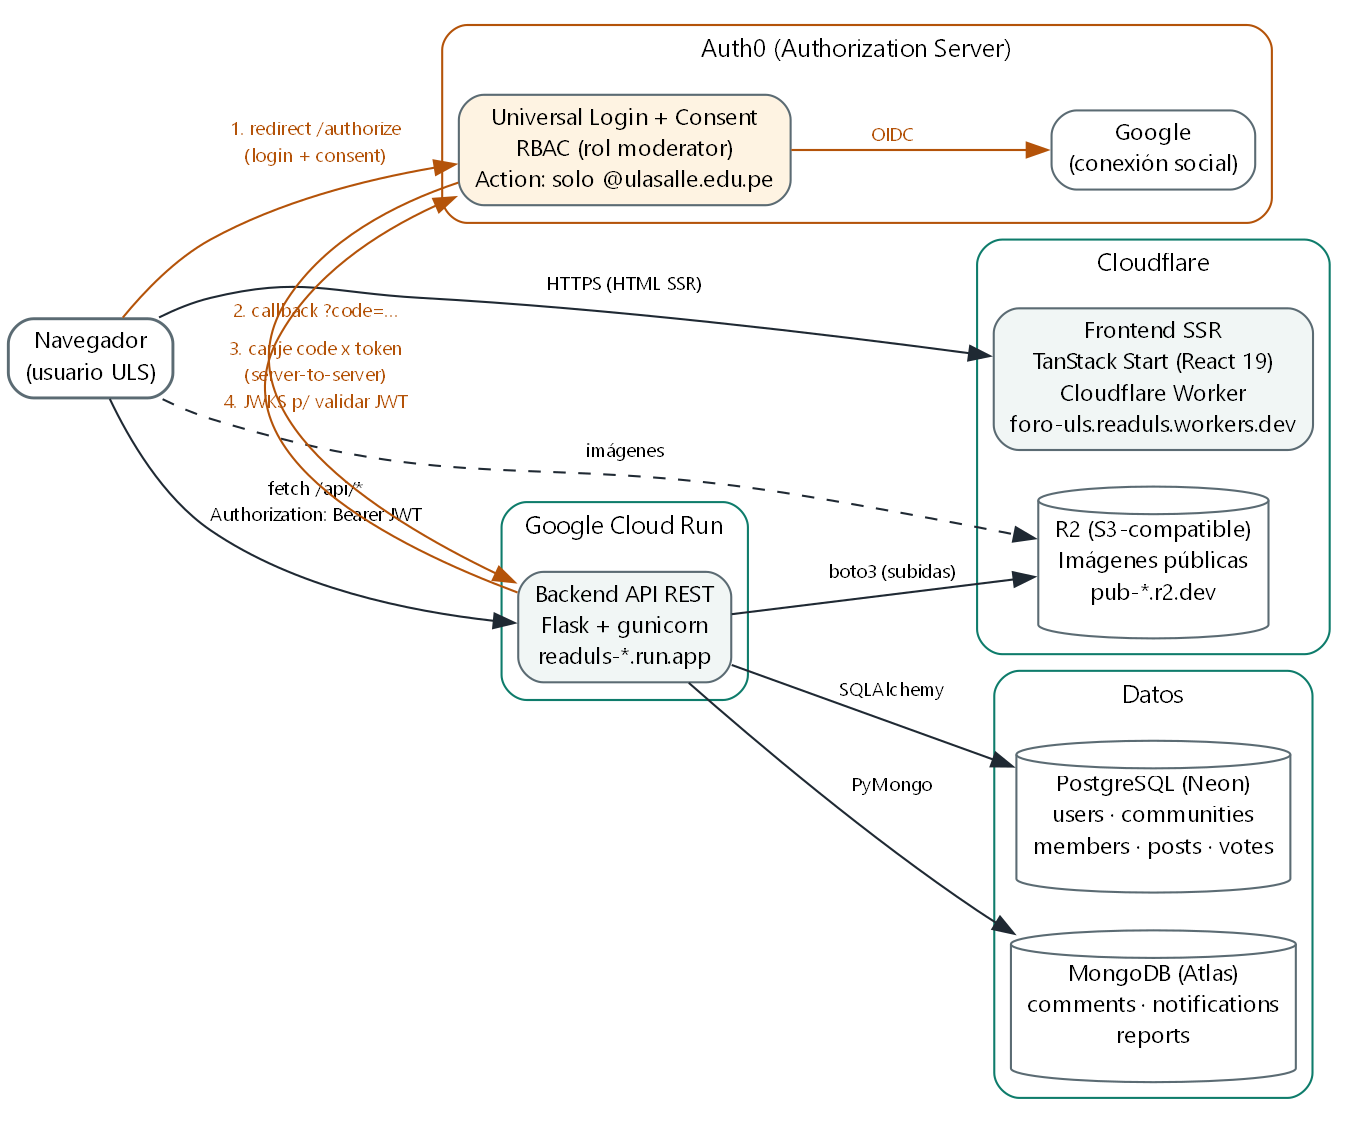
\includegraphics[width=\textwidth,keepaspectratio]{img/arquitectura.png}
    \caption{Arquitectura de componentes y flujo OAuth 2.0 (en naranja).}
    \label{fig:arq}
\end{figure}

\begin{table}[H]
\setlength{\tabcolsep}{0.4em}
{\renewcommand{\arraystretch}{1.3}
\begin{tabular}{|p{3cm}|p{6.6cm}|p{4.6cm}|}
    \hline
    \rowcolor{tablebackground}
    \color{white}\textbf{Capa} & \color{white}\textbf{Tecnología} & \color{white}\textbf{Hosting} \\
    \hline
    Frontend & TanStack Start (React 19, SSR) + Tailwind CSS v4 + shadcn/ui, empaquetado con Bun/Vite & Cloudflare Workers \\
    \hline
    Backend & Flask 3 (API REST) + SQLAlchemy + PyMongo, servido con gunicorn & Google Cloud Run \\
    \hline
    Autenticación & Auth0 — OAuth 2.0 Authorization Code + OIDC, RBAC & Auth0 (SaaS) \\
    \hline
    BD relacional & PostgreSQL & Neon \\
    \hline
    BD NoSQL & MongoDB & MongoDB Atlas \\
    \hline
    Objetos & Cloudflare R2 (S3-compatible, boto3) & Cloudflare \\
    \hline
\end{tabular}}
\caption{Stack tecnológico y plataformas de despliegue.}
\end{table}

% ==========================================================================
\section{Componente: Base de datos}

\subsection{Justificación del uso de dos bases de datos}

\begin{itemize}[itemsep=2pt]
    \item \textbf{PostgreSQL (relacional):} usuarios, carreras, comunidades,
    membresías, publicaciones y votos. Son datos estructurados con relaciones
    fuertes que exigen \textbf{integridad referencial}: un voto no puede
    existir sin su publicación y su usuario
    (\texttt{FOREIGN KEY} + \texttt{UNIQUE(post\_id, user\_id)}), una
    membresía es única por par comunidad-usuario, y las consultas del feed
    usan \textit{joins}.
    \item \textbf{MongoDB (NoSQL):} comentarios, notificaciones y reportes.
    Son \textbf{documentos flexibles de alta escritura}: los comentarios
    forman un árbol de profundidad arbitraria (\textit{materialized path} vía
    \texttt{parent\_id} + \texttt{depth}) que en SQL exigiría \textit{joins}
    recursivos costosos; las notificaciones y reportes tienen forma variable
    según el tipo y no necesitan transaccionalidad relacional.
\end{itemize}

\subsection{Modelo de datos}

\begin{figure}[H]
    \centering
    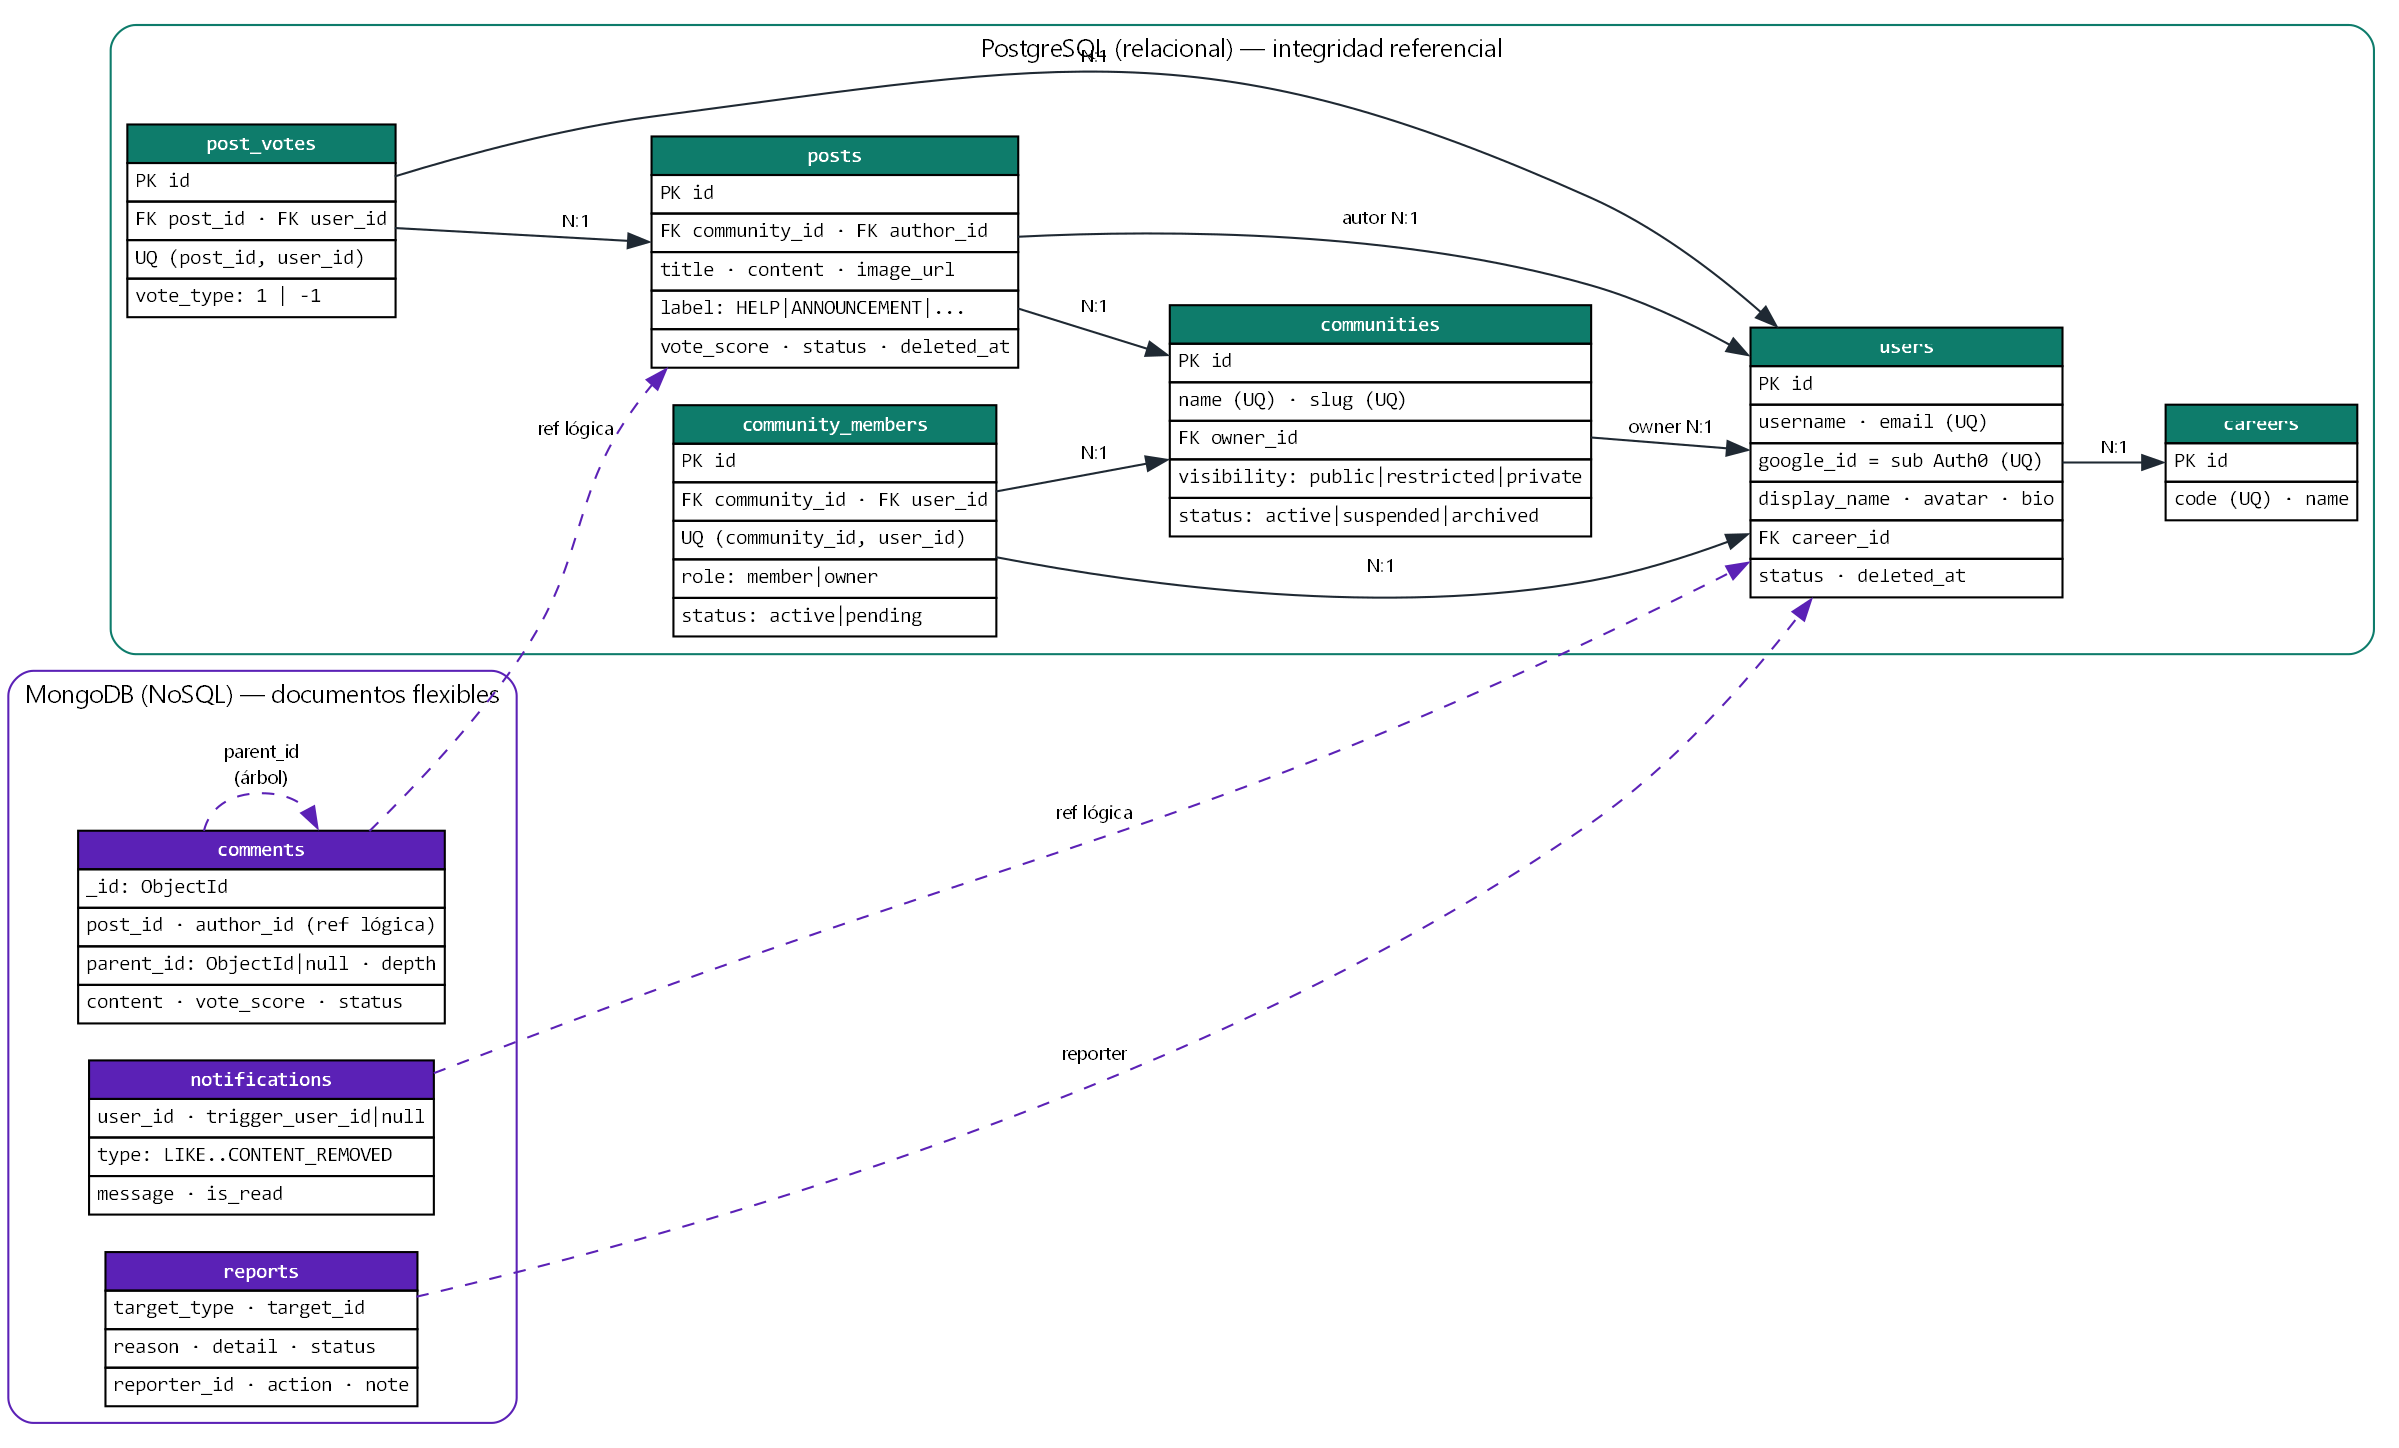
\includegraphics[width=\textwidth,keepaspectratio]{img/modelo_er.png}
    \caption{Modelo entidad–relación: tablas PostgreSQL (izquierda/arriba) y colecciones MongoDB con referencias lógicas (punteadas).}
    \label{fig:er}
\end{figure}

\subsection{Detalle de tablas y colecciones}

\textbf{PostgreSQL} (creadas por SQLAlchemy con \texttt{db.create\_all()} a
partir de \texttt{backend/models.py}):

\begin{table}[H]
\setlength{\tabcolsep}{0.4em}
{\renewcommand{\arraystretch}{1.25}
\begin{tabular}{|p{3.4cm}|p{11cm}|}
    \hline
    \rowcolor{tablebackground}
    \color{white}\textbf{Tabla} & \color{white}\textbf{Contenido y restricciones} \\
    \hline
    \texttt{users} & Perfil; \texttt{google\_id} guarda el \texttt{sub} de Auth0 (único); \textit{soft delete} con \texttt{deleted\_at}. \\
    \hline
    \texttt{careers} & Catálogo de carreras ULS (\texttt{code} único). \\
    \hline
    \texttt{communities} & \texttt{visibility}: public/restricted/private; \texttt{status}: active/suspended/archived; dueño con FK. \\
    \hline
    \texttt{community\_members} & N:M usuario-comunidad; \texttt{UNIQUE(community\_id, user\_id)}; \texttt{status} active/pending para el flujo de aprobación. \\
    \hline
    \texttt{posts} & Publicación con etiqueta, imagen, \texttt{vote\_score} desnormalizado y \textit{soft delete}. \\
    \hline
    \texttt{post\_votes} & Un voto por usuario y publicación (\texttt{UNIQUE}); \texttt{vote\_type} $\in \{1,-1\}$. \\
    \hline
\end{tabular}}
\end{table}

\textbf{MongoDB} (índices creados al arrancar, \texttt{backend/database.py}):

\begin{table}[H]
\setlength{\tabcolsep}{0.4em}
{\renewcommand{\arraystretch}{1.25}
\begin{tabular}{|p{3.4cm}|p{7.2cm}|p{3.8cm}|}
    \hline
    \rowcolor{tablebackground}
    \color{white}\textbf{Colección} & \color{white}\textbf{Contenido} & \color{white}\textbf{Índices} \\
    \hline
    \texttt{comments} & Árbol por \texttt{parent\_id} + \texttt{depth}; votos con \texttt{\$inc} atómico; \textit{soft delete}. & \texttt{(post\_id, parent\_id)}, \texttt{(post\_id, created\_at)} \\
    \hline
    \texttt{notifications} & 10 tipos; \texttt{trigger\_user\_id = null} para notificaciones anónimas de moderación. & \texttt{(user\_id, created\_at)} \\
    \hline
    \texttt{reports} & Reporte + resolución (\texttt{status}, \texttt{action}, \texttt{note}, \texttt{resolved\_by}). & \texttt{(status, created\_at)} \\
    \hline
\end{tabular}}
\end{table}

% ==========================================================================
\section{Componente: Backend (API REST)}

API Flask organizada en \textit{blueprints} por dominio
(\texttt{backend/routes/}): \texttt{auth}, \texttt{users},
\texttt{communities}, \texttt{posts}, \texttt{comments}, \texttt{reports},
\texttt{careers}, \texttt{uploads}.

\subsection{Convenciones REST y manejo de errores}

\begin{itemize}[itemsep=2pt]
    \item Códigos correctos: \texttt{200} lectura, \texttt{201} creación,
    \texttt{204} borrado, \texttt{400} validación, \texttt{401} sin token,
    \texttt{403} sin permiso, \texttt{404} no encontrado, \texttt{409} conflicto.
    \item Formato de error único en toda la API, incluidos los manejadores
    globales de \texttt{404/405/500} (nunca HTML de Flask):
\end{itemize}

\begin{lstlisting}[language=bash,caption={Shape de error consistente}]
{ "error": { "code": "FORBIDDEN",
             "message": "No autorizado: no eres el dueño de este recurso" } }
\end{lstlisting}

\subsection{Endpoints}

\begin{table}[H]
\setlength{\tabcolsep}{0.35em}
{\renewcommand{\arraystretch}{1.22}
\footnotesize
\begin{tabular}{|p{6.9cm}|p{2.1cm}|p{5.4cm}|}
    \hline
    \rowcolor{tablebackground}
    \color{white}\textbf{Endpoint} & \color{white}\textbf{Acceso} & \color{white}\textbf{Descripción} \\
    \hline
    \texttt{GET /api/auth/login} & Público & Inicia el flujo Authorization Code \\
    \hline
    \texttt{GET /oauth/callback} & Auth0 & Canjea el \texttt{code}, provisiona usuario \\
    \hline
    \texttt{GET /api/auth/me} & Bearer & Usuario autenticado (valida JWT) \\
    \hline
    \texttt{GET /api/auth/logout} & Público & Cierra sesión SSO en Auth0 \\
    \hline
    \texttt{GET /api/users}, \texttt{/api/users/:id} & Público & Listado y perfil \\
    \hline
    \texttt{PUT|DELETE /api/users/:id} & Dueño$^{*}$ & Editar / desactivar cuenta \\
    \hline
    \texttt{GET /api/users/:id/notifications} & Dueño & Notificaciones propias \\
    \hline
    \texttt{PATCH /api/users/:id/notifications/read} & Dueño & Marcar todas leídas \\
    \hline
    \texttt{GET /api/communities}, \texttt{/:id} & Público & Con \texttt{member\_count} y membresía \\
    \hline
    \texttt{POST /api/communities} & Bearer & Crear (privacidad configurable) \\
    \hline
    \texttt{PUT|DELETE /api/communities/:id} & Dueño$^{*}$ & Editar / archivar \\
    \hline
    \texttt{POST /api/communities/:id/join|leave} & Bearer & Unirse (según privacidad) / salir \\
    \hline
    \texttt{GET /api/communities/:id/members} & Público & Pendientes solo para el dueño \\
    \hline
    \texttt{PATCH|DELETE .../members/:user\_id} & Dueño & Aprobar / expulsar \\
    \hline
    \texttt{GET /api/posts}, \texttt{/:id}, \texttt{.../posts} & Público & Feed global, por comunidad, detalle \\
    \hline
    \texttt{POST /api/posts} & Bearer & Crear (autor = usuario del token) \\
    \hline
    \texttt{PUT|DELETE /api/posts/:id} & Dueño$^{*}$ & Editar / eliminar \\
    \hline
    \texttt{POST /api/posts/:id/vote} & Bearer & Votar (toggle, un voto por usuario) \\
    \hline
    \texttt{GET|POST /api/posts/:id/comments} & Púb./Bearer & Hilo de comentarios / comentar \\
    \hline
    \texttt{PUT|DELETE /api/comments/:id} & Dueño$^{*}$ & Editar / eliminar comentario \\
    \hline
    \texttt{POST /api/comments/:id/vote} & Bearer & Votar comentario \\
    \hline
    \texttt{POST /api/reports} & Bearer & Reportar contenido \\
    \hline
    \texttt{GET /api/reports} & Moderador & Bandeja con reportante visible \\
    \hline
    \texttt{PATCH /api/reports/:id} & Moderador & Resolver: banear/mantener/descartar + motivo \\
    \hline
    \texttt{GET /api/careers} & Público & Catálogo \\
    \hline
    \texttt{POST /api/uploads} & Bearer & Subir imagen, devuelve URL pública \\
    \hline
\end{tabular}}
\caption{Endpoints de la API. $^{*}$ = el moderador (rol Auth0) también puede.}
\end{table}

% ==========================================================================
\section{Componente: Frontend}

SPA con \textbf{Server-Side Rendering} (TanStack Start / React 19) desplegada
como Cloudflare Worker: el servidor renderiza el \textit{shell} completo de la
aplicación y la metadata SEO/OpenGraph en cada petición; los datos de la API
se cargan en el cliente con TanStack Query tras la hidratación.

\subsection{Páginas}

\begin{table}[H]
\setlength{\tabcolsep}{0.4em}
{\renewcommand{\arraystretch}{1.22}
\footnotesize
\begin{tabular}{|p{5.2cm}|p{9.2cm}|}
    \hline
    \rowcolor{tablebackground}
    \color{white}\textbf{Ruta} & \color{white}\textbf{Página} \\
    \hline
    \texttt{/login}, \texttt{/oauth/callback} & Login (botón único Auth0) y recepción del token \\
    \hline
    \texttt{/} , \texttt{/feed/label/:label}, \texttt{/feed/career/:code}, \texttt{/feed/announcements} & Feed global y filtrado por etiqueta, carrera o anuncios \\
    \hline
    \texttt{/communities}, \texttt{/communities/create} & Listado y creación con selector de privacidad \\
    \hline
    \texttt{/communities/:id}, \texttt{/:id/members}, \texttt{/:id/edit} & Detalle con unirse/salir, miembros con aprobación, edición \\
    \hline
    \texttt{/publications/:id}, \texttt{/:id/edit} & Detalle con hilo de comentarios, votos, reporte; edición \\
    \hline
    \texttt{/users/:id}, \texttt{/users/:id/settings} & Perfil público; configuración \textbf{solo del propio usuario} \\
    \hline
    \texttt{/notifications} & Campana: sociales (con avatar) y de moderación (anónimas) \\
    \hline
    \texttt{/moderation} & Panel de moderación (solo rol \texttt{moderator}) \\
    \hline
    \texttt{/bookmarks}, \texttt{/search}, \texttt{/rules}, \texttt{/onboarding} & Guardados, búsqueda, reglas, primer inicio \\
    \hline
\end{tabular}}
\caption{Rutas del frontend (TanStack Router, file-based).}
\end{table}

\subsection{Sesión y protección en el cliente}

\begin{itemize}[itemsep=2pt]
    \item El cliente HTTP central adjunta \texttt{Authorization: Bearer
    <access\_token>} en cada petición; un \texttt{401} limpia la sesión local.
    \item \textit{Guards} de ruta: \texttt{requireAuth} (exige sesión) y
    \texttt{requireSelf} (rutas personales: cambiar el id en la URL redirige a
    la propia), con re-verificación dentro del componente como defensa en
    profundidad.
    \item \texttt{isModerator()} decodifica el claim de roles del JWT solo
    para decidir qué UI mostrar; la autorización real siempre la aplica el
    backend.
    \item La interfaz refleja \textbf{login/logout} y muestra solo los datos
    del usuario autenticado (notificaciones, configuración, acciones de dueño).
\end{itemize}

% ==========================================================================
\section{Componente: Autenticación y autorización (OAuth 2.0)}

\subsection{Proveedor elegido y justificación}

Se eligió \textbf{Auth0} como Authorization Server de terceros porque: (a)
implementa OAuth 2.0/OIDC estándar con Universal Login y pantalla de
consentimiento hospedadas; (b) permite mantener el acceso con Google
institucional como conexión social \textit{detrás} del proveedor, con una
\textit{Action} que rechaza cuentas fuera de \texttt{@ulasalle.edu.pe}; (c)
provee \textbf{RBAC} para delegar también la autorización (rol
\texttt{moderator} inyectado en el token); y (d) su capa gratuita cubre el
alcance del proyecto sin tarjeta de crédito.

\subsection{Flujo Authorization Code end-to-end}

\begin{enumerate}[itemsep=2pt]
    \item El usuario pulsa \textit{Iniciar sesión} en el frontend $\rightarrow$
    \texttt{GET /api/auth/login} redirige a
    \texttt{https://\{tenant\}.auth0.com/authorize} con
    \texttt{response\_type=code}, \texttt{client\_id},
    \texttt{redirect\_uri}, \texttt{scope=openid profile email},
    \texttt{audience} y \texttt{state} (anti-CSRF).
    \item Auth0 muestra login + consentimiento (Google institucional detrás);
    la Action \textit{post-login} bloquea dominios no institucionales.
    \item Auth0 redirige al backend (\texttt{/oauth/callback}) con el
    \texttt{code}; el backend verifica el \texttt{state} y canjea el código
    \textbf{server-to-server} en \texttt{/oauth/token} usando el
    \texttt{client\_secret} (nunca expuesto al navegador).
    \item El backend recibe el \texttt{access\_token} (JWT RS256), provisiona
    el usuario local por su \texttt{sub} y lo entrega al frontend en el
    \textit{fragmento} de la URL (que no viaja a servidores y se elimina de la
    barra de direcciones inmediatamente).
    \item En cada petición protegida, el backend valida el JWT contra el
    \textbf{JWKS} del tenant (llaves públicas cacheadas): firma,
    \texttt{aud} (= \texttt{AUTH0\_AUDIENCE}), \texttt{iss} y \texttt{exp}.
    \item \textbf{Ownership por \texttt{sub}}: la identidad se resuelve
    únicamente desde el token validado; el autor de cada recurso creado es el
    usuario del token (se ignora cualquier id enviado por el cliente), y
    editar/borrar recursos ajenos responde \texttt{403}.
    \item \textbf{Logout} completo: limpia la sesión local y cierra la sesión
    SSO en Auth0 (\texttt{/v2/logout}), permitiendo reintentar con otra
    cuenta (también tras un rechazo por dominio).
\end{enumerate}

\begin{lstlisting}[language=Python,caption={Validación del access token por JWKS (backend/auth\_utils.py)}]
_jwk_client = PyJWKClient(f"https://{AUTH0_DOMAIN}/.well-known/jwks.json")

def verify_access_token(token):
    signing_key = _jwk_client.get_signing_key_from_jwt(token).key
    return jwt.decode(token, signing_key, algorithms=["RS256"],
                      audience=AUTH0_AUDIENCE, issuer=_ISSUER)

def current_user():
    claims = verify_access_token(_bearer_token())
    return User.query.filter_by(google_id=claims["sub"],
                                deleted_at=None).first()
\end{lstlisting}

\subsection{Autorización por roles (RBAC)}

El rol \texttt{moderator} se administra en Auth0 (User Management
$\rightarrow$ Roles) y una Action lo inyecta en el token como claim
\textit{namespaced} (\texttt{https://readuls/roles}). El decorador
\texttt{@require\_moderator} protege la bandeja de reportes y las acciones de
moderación; \texttt{forbid\_unless\_owner\_or\_moderator} permite al moderador
retirar o editar contenido ajeno (siempre notificando al autor).

\subsection{Configuración en variables de entorno}

Ninguna credencial está \textit{hardcodeada}; todo vive en \texttt{.env}
(ignorado por git) con plantillas \texttt{.env.example} versionadas:

\begin{table}[H]
\setlength{\tabcolsep}{0.4em}
{\renewcommand{\arraystretch}{1.25}
\footnotesize
\begin{tabular}{|p{4.6cm}|p{9.8cm}|}
    \hline
    \rowcolor{tablebackground}
    \color{white}\textbf{Variable} & \color{white}\textbf{Uso} \\
    \hline
    \texttt{AUTH0\_DOMAIN} & Tenant del Authorization Server \\
    \hline
    \texttt{AUTH0\_CLIENT\_ID / \_SECRET} & Credenciales del cliente OIDC (canje server-to-server) \\
    \hline
    \texttt{AUTH0\_AUDIENCE} & Identifier de la API en Auth0 (hace que el token sea JWT) \\
    \hline
    \texttt{AUTH0\_CALLBACK\_URL} & Redirect URI registrada en Auth0 \\
    \hline
    \texttt{AUTH0\_ROLES\_CLAIM} & Claim namespaced de roles (RBAC) \\
    \hline
    \texttt{POSTGRES\_URL / MONGO\_URL} & Conexiones a Neon y Atlas \\
    \hline
    \texttt{AWS\_*} & Credenciales y endpoint del almacenamiento S3-compatible \\
    \hline
    \texttt{FLASK\_SECRET\_KEY / FRONTEND\_URL} & Sesión de Flask (state OAuth) y retorno al frontend \\
    \hline
\end{tabular}}
\caption{Variables de entorno principales (ver \texttt{backend/.env.example}).}
\end{table}

% ==========================================================================
\section{Moderación y notificaciones}

\subsection{Ciclo de un reporte}
\begin{enumerate}[itemsep=1pt]
    \item Un usuario reporta una publicación o comentario (motivo + detalle).
    \item El autor del contenido recibe una notificación \textbf{anónima}:
    \textit{«Alguien ha reportado tu publicación por el motivo ... »} — nunca
    se revela quién reportó.
    \item El moderador ve el reporte en el panel (con el nombre del
    reportante) y lo resuelve con motivo adjunto: \textbf{eliminar} el
    contenido (\textit{soft delete}), \textbf{mantener} o \textbf{descartar}.
    \item Reportante y autor reciben el veredicto con el motivo del moderador.
\end{enumerate}

\subsection{Tipos de notificación}

\begin{table}[H]
\setlength{\tabcolsep}{0.4em}
{\renewcommand{\arraystretch}{1.22}
\footnotesize
\begin{tabular}{|p{3.9cm}|p{6cm}|p{2.6cm}|p{1.6cm}|}
    \hline
    \rowcolor{tablebackground}
    \color{white}\textbf{Tipo} & \color{white}\textbf{Se dispara cuando} & \color{white}\textbf{Destinatario} & \color{white}\textbf{Anónima} \\
    \hline
    \texttt{LIKE} / \texttt{DISLIKE} & Votan tu publicación & Autor & No \\
    \hline
    \texttt{COMMENT} & Comentan tu publicación & Autor del post & No \\
    \hline
    \texttt{REPLY} & Responden tu comentario & Autor del padre & No \\
    \hline
    \texttt{COMMUNITY\_POST} & Nueva publicación en tu comunidad & Miembros & No \\
    \hline
    \texttt{ANNOUNCEMENT} & Anuncio en tu comunidad & Miembros & No \\
    \hline
    \texttt{REPORT\_RECEIVED} & Reportan tu contenido & Autor & \textbf{Sí} \\
    \hline
    \texttt{REPORT\_RESOLVED} & Se resuelve un reporte & Reportante y autor & Parcial \\
    \hline
    \texttt{CONTENT\_REMOVED} & Un moderador banea tu contenido & Autor & \textbf{Sí} \\
    \hline
    \texttt{CONTENT\_EDITED} & Un moderador edita tu contenido & Autor & \textbf{Sí} \\
    \hline
\end{tabular}}
\caption{Cobertura del sistema de notificaciones.}
\end{table}

% ==========================================================================
\section{Componente: Despliegue}

\begin{itemize}[itemsep=2pt]
    \item \textbf{Backend} en Google Cloud Run: despliegue desde código fuente
    (\texttt{gcloud run deploy readuls --source backend}); Cloud Build
    construye el \texttt{Dockerfile} (gunicorn, \texttt{\$PORT} inyectado).
    Escala a cero (arranque en frío de 1–3 s).
    \item \textbf{Frontend} en Cloudflare Workers:
    \texttt{bun run build} + \texttt{wrangler deploy}. La URL de la API se
    fija en tiempo de build (\texttt{VITE\_API\_BASE\_URL}).
    \item \textbf{Datos gestionados}: Neon (PostgreSQL, TLS obligatorio),
    MongoDB Atlas (M0, cadena SRV) y Cloudflare R2 (imágenes públicas).
    \item \textbf{Desarrollo local}: \texttt{docker compose up} levanta
    Postgres, MongoDB, MinIO (S3 local), backend y frontend.
    \item Guía completa paso a paso en \texttt{docs/DEPLOY.md}.
\end{itemize}

\begin{lstlisting}[language=bash,caption={Comandos de despliegue}]
# Backend -> Cloud Run (construye el Dockerfile con Cloud Build)
gcloud run deploy readuls --source backend --region us-central1 \
      --env-vars-file env.yaml

# Frontend -> Cloudflare Workers
cd frontend && bun run build
bunx wrangler deploy -c .output/server/wrangler.json --name foro-uls
\end{lstlisting}

% ==========================================================================
\section{Entregables y cumplimiento de la rúbrica}

\begin{table}[H]
\setlength{\tabcolsep}{0.4em}
{\renewcommand{\arraystretch}{1.25}
\footnotesize
\begin{tabular}{|p{3.2cm}|p{11.4cm}|}
    \hline
    \rowcolor{tablebackground}
    \color{white}\textbf{Entregable} & \color{white}\textbf{Evidencia} \\
    \hline
    Repositorio Git & \url{\repoUrl} — backend + frontend + bd + docs, con historial de commits del grupo. \\
    \hline
    README.md & Tema, arquitectura, proveedor OAuth y justificación, justificación de las 2 BD, cómo correr todo; README técnico adicional por módulo. \\
    \hline
    .env.example & \texttt{backend/.env.example} y \texttt{frontend/.env.example} con todas las variables y placeholders. \\
    \hline
    Postman & \texttt{postman\_collection.json}: carpetas \textit{Público}, \textit{Autenticado (Bearer)}, \textit{Moderador} y \textit{Errores esperados} (401/403/404), con variables \texttt{base\_url} y \texttt{token}. \\
    \hline
    Diagrama & Figuras \ref{fig:arq} (arquitectura + flujo OAuth) y \ref{fig:er} (modelo de datos). \\
    \hline
    Demo en vivo & \url{\frontUrl} (frontend) y \url{\apiUrl} (API). \\
    \hline
\end{tabular}}
\caption{Entregables del trabajo final.}
\end{table}

\begin{table}[H]
\setlength{\tabcolsep}{0.4em}
{\renewcommand{\arraystretch}{1.25}
\footnotesize
\begin{tabular}{|p{4.1cm}|x{1cm}|p{9.6cm}|}
    \hline
    \rowcolor{tablebackground}
    \color{white}\textbf{Criterio} & \color{white}\textbf{Pts} & \color{white}\textbf{Cómo se cumple} \\
    \hline
    Backend y API & 4 & API REST funcional en producción; códigos HTTP correctos (200/201/204/400/401/403/404/409); formato de error único + manejadores globales. \\
    \hline
    Bases de datos & 3 & PostgreSQL y MongoDB en uso efectivo con modelo coherente y justificación documentada (sección 4 y README). \\
    \hline
    OAuth Authorization Code & 5 & Flujo completo end-to-end con Auth0; canje server-to-server; validación JWT por JWKS en cada request protegido; ownership por \texttt{sub}; config 100\% en \texttt{.env}. \\
    \hline
    Frontend & 3 & SSR con TanStack Start; consume la API; login/logout reflejados; solo datos del usuario autenticado (guards + backend). \\
    \hline
    Colección Postman & 2 & Todos los requests públicos y protegidos, incluyendo casos 401/403/404. \\
    \hline
    Documentación & 1 & README ejecutable + \texttt{.env.example} + diagramas + guía de despliegue. \\
    \hline
    Código y Git & 1 & Estructura modular por dominio; commits descriptivos distribuidos en el grupo. \\
    \hline
    Presentación & 1 & Aplicación corriendo en vivo en las URLs indicadas. \\
    \hline
\end{tabular}}
\caption{Trazabilidad contra la rúbrica de evaluación (20 pts).}
\end{table}

% ==========================================================================
\section{Cómo ejecutar el proyecto}

\begin{lstlisting}[language=bash,caption={Arranque local con Docker}]
cp backend/.env.example backend/.env    # completar AUTH0_* y FLASK_SECRET_KEY
cp frontend/.env.example frontend/.env
docker compose up -d --build
# Frontend: http://localhost:8080  |  Backend: http://localhost:5000
\end{lstlisting}

Para probar la API sin frontend: importar \texttt{postman\_collection.json},
iniciar sesión en la app y copiar el token \texttt{auth\_token} desde el
\textit{localStorage} del navegador a la variable \texttt{token} de Postman.

\section{Conclusiones}

\begin{itemize}[itemsep=2pt]
    \item Delegar la autenticación a un Authorization Server de terceros
    (Auth0) simplificó el sistema y elevó su seguridad: la aplicación nunca
    maneja contraseñas, y la validación por JWKS ancla cada petición a una
    identidad verificada criptográficamente.
    \item La separación relacional/NoSQL respondió a criterios técnicos
    verificables: integridad referencial para el dominio estructurado y
    documentos flexibles para árboles de comentarios, notificaciones y
    reportes de alta escritura.
    \item El \textit{ownership} por \texttt{sub} y el RBAC delegado
    demostraron que autorización y autenticación pueden externalizarse sin
    perder control fino en la API (401/403 correctos y verificables en Postman).
    \item El despliegue en capas gratuitas gestionadas (Cloud Run, Cloudflare,
    Neon, Atlas) permitió operar una aplicación completa en producción sin
    costo, con la única concesión del arranque en frío.
\end{itemize}

\clearpage
\section{Referencias}
\begin{itemize}
    \item \url{https://auth0.com/docs/get-started/authentication-and-authorization-flow/authorization-code-flow}
    \item \url{https://datatracker.ietf.org/doc/html/rfc6749} — The OAuth 2.0 Authorization Framework
    \item \url{https://flask.palletsprojects.com/}
    \item \url{https://tanstack.com/start}
    \item \url{https://www.mongodb.com/docs/manual/applications/data-models-tree-structures/}
    \item \url{https://cloud.google.com/run/docs}
    \item \url{https://developers.cloudflare.com/workers/}
\end{itemize}

\end{document}
